\section{What computation can reach, and what the sine squared lemma adds}\label{ch:motivation}
\label{sec:motivation}


Two facts govern what computation can establish about the Thorin condition and which evaluator it should use. A finite computation that finds no zero off the line cannot by itself measure a distance to RH: on a window where the zeros have been counted it reproduces $U_{\RH}$, and at a stated resolution it measures the positivity margin of $\rho_\varepsilon$ up to a stated height, but neither result constrains the zeros above the window (Section~\ref{sec:ch6:measure}). The sine squared lemma identifies the Thorin density from the primes but is a poor way to compute it: its pole and prime pieces cancel as the basepoint approaches one, below one its prime sum diverges, and near the critical line the smoothed prime sum that replaces it needs a number of primes exponential in $1/\varepsilon$ (Section~\ref{sec:ch6:split}). The P\'olya density has none of these defects, and it is the evaluator in the rest of this chapter and in Chapters~\ref{chap:hcm} and \ref{chap:heat}. The lemma still shapes the computations: it makes the cumulative Thorin mass an argument, it poses positivity certificates as linear programs whose only negative input is the pole, and it gives an exact consistency check at the centre (Section~\ref{sec:ch6:consequences}).

\subsection{What a finite computation can measure}\label{sec:ch6:measure}

On a window where the zeros have been counted, computation identifies the Thorin functional with $U_{\RH}$. Below height $200$ the P\'olya route finds $79$ sign changes of $\Xi$ and an argument principle count $N(200)=79.0000000000004$ (Section~\ref{sec:ch4:height200}). So, numerically and in agreement with \cite{Backlund,PT21}, the $79$ zeros below height $200$ are simple and on the line, and the Thorin functional $U=\sum_k\delta_{a_k}$ of Section~\ref{ch:arith} coincides with $U_{\RH}$ on $(0,200^2]$. The matched total variation distance of Section~\ref{ch:distances}, computed against a model of the zero list, is $3.7\times10^{-9}\,\varepsilon$ at every resolution computed, the numerical floor of the comparison.

None of this constrains the zeros above the window. Platt and Trudgian \cite{PT21} have verified every zero below height $3\times10^{12}$, yet the perturbation of $\xi$ in Theorem~\ref{thm:ch13:perturb} \cite[Chapter 11]{P26} keeps the order, type and symmetry of $\xi(\tfrac12+s)$, puts zeros off the line just above any large enough height $R$ for which RH has been verified up to $R+50$, and still passes the finite tests of the heat trace, from Hankel blocks and derivative signs (to order $10^{17}$) to the small time expansion. Tests that count zeros find such a perturbation only when they reach its height. So a computation from the zeros verified up to a given height, or from finitely many tests of the heat trace, cannot by itself measure a scalar distance to RH, although a finite computation could refute RH by certifying a zero off the line. What it can measure is a margin at a stated resolution and height.

The margin is the minimum of $\rho_\varepsilon$, and positivity on one line is weaker than a zero free half plane. If every zero has real part less than $\tfrac12+\varepsilon$, then $\rho_\varepsilon>0$ and the reciprocal at basepoint $\tfrac12+\varepsilon$ is a GGC transform with Thorin measure $\mu_\varepsilon$ (Theorem~\ref{thm:poisson}), so a negative value of $\rho_\varepsilon$ proves a zero to the right of the line. The converse is not known for $\xi$, because the positive kernels of the other zeros can outweigh the negative kernel of a zero to the right of the line (Remark~\ref{rem:ch2:oneline}); Section~\ref{sec:ch13:visibility} states, to first order in $\varepsilon$, when they cannot. Positivity on every line $\re s=\tfrac12+\varepsilon'$ with $\varepsilon'>\varepsilon$ does exclude such zeros, and positivity for every $\varepsilon>0$ is Lagarias's criterion \cite{Lagarias}, which is RH.

Resolution is the first limitation. On $0\le\theta\le200$ the computed minimum is $\min\rho_\varepsilon=0.0147\,\varepsilon$ at each of the eight resolutions of Section~\ref{sec:ch4:height200}, attained at $\theta=0$, where $\rho_\varepsilon(0)=\pi^{-1}\xi'(\tfrac12+\varepsilon)/\xi(\tfrac12+\varepsilon)=2\varepsilon\pi^{-1}\sum_ka_k^{-1}+O(\varepsilon^3)$, because $(\xi'/\xi)(\tfrac12+\varepsilon)=\sum_k2\varepsilon/(\varepsilon^2+a_k)$ and $\sum_k a_k^{-1}=0.0231050$ (Section~\ref{ch:clock}). So $\inf_\theta\rho_\varepsilon(\theta)\le\rho_\varepsilon(0)\to0$ as $\varepsilon\downarrow0$: near the critical line positivity is never won by a fixed margin, and nothing in a finite window prevents it from failing above the window. On the verified window the origin is in fact the minimum: for every $\varepsilon\in(0,6.85]$ the minimum of $\rho_\varepsilon$ over $0\le\theta\le3\times10^{12}-1.21$ is $\rho_\varepsilon(0)$, attained only at the origin, and that this holds at every height for every $\varepsilon\in(0,\frac12)$ is equivalent to RH (Theorem~\ref{thm:dbeta:minall} and Remark~\ref{rem:dbeta:margin}).

Height is the second limitation. The untilted P\'olya route loses about $\pi\theta/(4\log10)=0.341\,\theta$ decimal digits at height $\theta$, because $|\xi(\tfrac12+\varepsilon+i\theta)|$ decays like $e^{-\pi\theta/4}$, up to a power of $\theta$, while the integrands are of order one; height $10^4$ would require about $3400$ digits per point. The tilted contour of Section~\ref{sec:newcomp}, at distance $\delta$ from the edge of the strip of analyticity of $\Phi$, reduces the loss to about $\delta\theta/\log10$ digits and gives $25$ digits of $\rho_{0.05}$ at height $5000$ in $28$ milliseconds per point (Table~\ref{tab:tilt}), but the number of nodes, and with it the cost per point, still grows linearly in the height. The Riemann Siegel formula and the Odlyzko Sch\"onhage algorithm evaluate $\zeta$ at large height far more cheaply (Section~\ref{ch:classical}), so the P\'olya route is not a competitor for zero verification; the division of labour between the two is drawn at the end of Section~\ref{sec:ch5:count}. Its value is accuracy at small $\varepsilon$ on moderate windows, where the Thorin measure is sharp and the prime side is ill conditioned.

\subsection{The sine squared decomposition of the Thorin bracket}\label{sec:ch6:split}

The sine squared lemma \eqref{eq:sin2} converts the L\'evy description of $\log\xi$, in which the primes are atoms, into the Thorin description of the reciprocal, in which each zero contributes a Poisson kernel (Proposition~\ref{prop:struct}) and becomes an atom only in the limit $\varepsilon\downarrow0$ under RH. At a basepoint $\alpha>1$, applying the kernel $2\sin^2(x\theta/2)=1-\cos(x\theta)$ to the canonical measure of \cite[Theorem 8.1]{P26} writes the bracket $v_\alpha(\theta)=\re(\xi'/\xi)(\alpha+i\theta)$ as a sum of four explicit pieces:
\begin{multline}\label{eq:split}
v_\alpha(\theta)=\underbrace{\frac{\xi'}{\xi}(\alpha)}_{\text{drift}}+\underbrace{\int_0^\infty(1-\cos\theta x)\frac{e^{-\alpha x}}{e^{2x}-1}\,dx}_{\text{archimedean}\ \ge0}\\
-\underbrace{\frac{\theta^2}{(\alpha-1)\big((\alpha-1)^2+\theta^2\big)}}_{\text{pole}\ \ge0}+\underbrace{\sum_{n\ge2}\frac{\Lambda(n)}{n^\alpha}\big(1-\cos(\theta\log n)\big)}_{\text{primes}\ \ge0}.
\end{multline}
The pole piece is the closed form of $\int_0^\infty(1-\cos\theta x)e^{-(\alpha-1)x}dx$, and the prime piece equals $-\tfrac{\zeta'}{\zeta}(\alpha)+\re\tfrac{\zeta'}{\zeta}(\alpha+i\theta)$.

The drift is the linear coefficient $c=\xi'/\xi(\alpha)$ of the L\'evy representation of Section~\ref{ch:clock}, not the drift $d$ of a GGC. The archimedean piece is the contribution of $\Gamma(s/2)$ together with the factor $s$ of $\frac12s(s-1)$; it is smooth in $\theta$ and grows like $\frac12\log\theta$, which accounts for the average density of zeros. The pole piece comes from the pole of $\zeta$ at $s=1$. The prime piece is a sum of oscillations with frequencies $\log n$ and amplitudes $\Lambda(n)n^{-\alpha}$, one for each prime power. The drift is positive, the archimedean and prime pieces are nonnegative, and only the pole piece enters with a minus sign.

Near $\alpha=1$ the pole piece is almost cancelled by the prime piece. At $\alpha=1.5$ and $\theta=2$ the pole contributes $-1.8824$ and the primes $+1.7683$, while $v_{1.5}(2)=0.0470$ (Table~\ref{tab:split} and Figure~\ref{fig:ch6:pieces}); the four columns of the table sum to $0.0457$, the difference $1.3\times10^{-3}$ being the prime tail beyond $2\times10^6$. Both pieces grow like $1/(\alpha-1)$, the pole explicitly and the primes through the pole of $-\zeta'/\zeta$ at one. At each fixed $\theta\ne0$ their difference stays bounded as $\alpha\downarrow1$ because $\zeta$ has no zero on the line $\re s=1$, so the analytic input of the prime number theorem appears in the Thorin description as this cancellation, which \cite[Section 8.2]{P26} identifies with the collapse onto the zeros. Measured by the condition number
\[
\kappa_\alpha(\theta)=\frac{|\text{pole}|+|\text{primes}|}{|v_\alpha(\theta)|},
\]
the prime side amplifies relative errors by $3.9$ at $\alpha=3$, $21.5$ at $\alpha=2$ and $77.6$ at $\alpha=1.5$, all at $\theta=2$. As $\alpha\downarrow1$ the numerator grows like $2/(\alpha-1)$ while $v_\alpha$ stays bounded.

\begin{table}[t]
\centering\small
\begin{tabular}{rrrrrrrr}
\toprule
$\alpha$ & $\theta$ & drift & archimedean & pole & primes & $v_\alpha(\theta)$ & $\kappa_\alpha(\theta)$\\
\midrule
3.0 & 2 & 0.1144 & 0.0533 & $-0.2500$ & 0.1988 & 0.1165 & 3.85\\
3.0 & 50 & 0.1144 & 1.2594 & $-0.4992$ & 0.2464 & 1.1210 & 0.67\\
2.0 & 2 & 0.0691 & 0.0859 & $-0.8000$ & 0.7154 & 0.0704 & 21.5\\
2.0 & 50 & 0.0691 & 1.3989 & $-0.9996$ & 0.7561 & 1.2245 & 1.43\\
1.5 & 2 & 0.0461 & 0.1137 & $-1.8824$ & 1.7683 & 0.0470 & 77.6\\
1.5 & 50 & 0.0461 & 1.4863 & $-1.9998$ & 1.8527 & 1.3867 & 2.78\\
\bottomrule
\end{tabular}
\caption{The four pieces of the sine squared decomposition \eqref{eq:split}, with the prime sum over $n\le2\times10^6$, and the bracket $v_\alpha(\theta)$ computed by the P\'olya route; it differs from the sum of the four columns by the prime tail beyond $2\times10^6$ ($1.3\times10^{-3}$ at $\alpha=1.5$, $\theta=2$). The pole column is the signed contribution, minus the pole piece. The pole and prime pieces grow like $1/(\alpha-1)$ and cancel to leave a bracket of order one or smaller; $\kappa_\alpha$ measures the loss.}
\label{tab:split}
\end{table}

\begin{figure}[htbp]
\centering
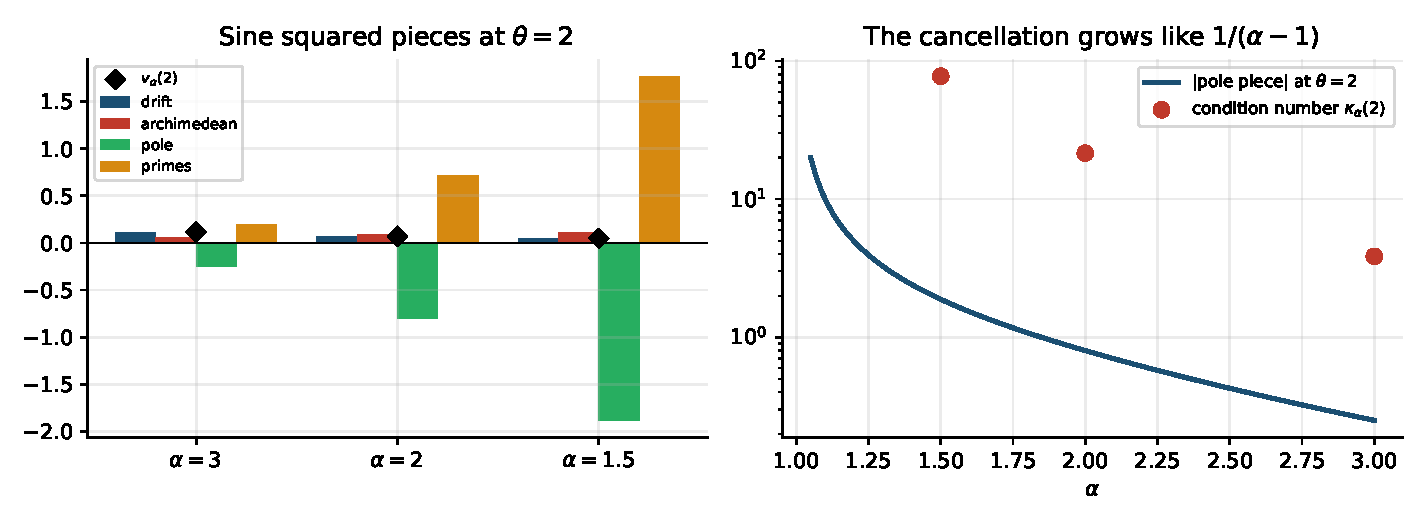
\includegraphics[width=\textwidth]{fig/sin2pieces.pdf}
\caption{Left: the four pieces of the sine squared decomposition at $\theta=2$ for three basepoints, with the bracket $v_\alpha(2)$. Right: the pole piece and the condition number grow like $1/(\alpha-1)$ as the basepoint approaches one.}
\label{fig:ch6:pieces}
\end{figure}

The lemma also prices the prime side. By the prime number theorem the truncation tail satisfies, for fixed $\theta\ne0$,
\[
\sum_{n>N}\frac{\Lambda(n)}{n^\alpha}\big(1-\cos(\theta\log n)\big)\asymp\frac{N^{1-\alpha}}{\alpha-1},
\]
which is $1.4\times10^{-3}$ at $\alpha=1.5$ with $N=2\times10^6$, the size of the errors in Table~\ref{tab:prime}; an absolute error of $10^{-10}$ at $\alpha=1.5$ would need a cutoff $N\approx4\times10^{20}$. For $\alpha\le1$ the series diverges, and the lemma must be read through the regularised pairing of \cite[Chapter 7]{P26} and the explicit formula. At the basepoint one the regularisation is explicit: the pole and prime pieces can be compensated against each other, and Section~\ref{ch:basepoint} converts the resulting L\'evy form of $\xi(1+s)$ term by term into the Thorin density. Near the critical line Selberg's smoothed sum over the primes up to $x^2$ takes the place of the series, and at resolution $\varepsilon$, if no zero lies to the right of the critical line, its error at an ordinate is of order $x^{-\varepsilon}/(\varepsilon^2\log x)$, so that $k$ correct digits need $x\approx10^{k/\varepsilon}$ (Section~\ref{sec:ch10:selberg}). The P\'olya route has none of these costs: its cost per point is polynomial in the height and independent of $\varepsilon$, and at height $200$ it reaches $\varepsilon=0.005$ with about $60$ digits (Section~\ref{sec:ch4:trapezoid}).

\subsection{Consequences for computation}\label{sec:ch6:consequences}

The bracket is the derivative of an argument, $v_\alpha(\theta)=\partial_\theta\arg\xi(\alpha+i\theta)$, because $\partial_\theta\log\xi(\alpha+i\theta)=i(\xi'/\xi)(\alpha+i\theta)$. So the cumulative Thorin mass is an argument,
\[
\mu_\varepsilon\big((0,\theta^2]\big)=\frac1\pi\arg\xi\Big(\frac12+\varepsilon+i\theta\Big),
\]
continued along the line from the real axis, where $\xi>0$. It is computed without quadrature, by accumulating the arguments of quotients of consecutive values of $\xi$, with steps chosen so that each increment can be read from its principal value, a condition checked after the fact rather than guaranteed (Section~\ref{sec:ch4:height200}). Section~\ref{ch:distances} uses it for masses, cell masses, cumulative distances and the mass defect of Proposition~\ref{prop:mass}, and Section~\ref{ch:turing} for the zero count.

The lemma is linear with a nonnegative kernel, so a nonnegative L\'evy input gives a nonnegative Thorin output, and positivity certificates can be posed as linear programs in the sine squared basis \cite[Sections 18.2.8 and 18.2.9]{P26}. For $\xi$ the only negative part of the input $xL(dx)$ is the pole density $-e^{-(\alpha-1)x}dx$, so a certificate must show that the positive pieces dominate the pole piece at every $\theta$. For $\alpha>1$ they do (Theorem~\ref{thm:poisson}), although the proof goes through the zeros and not through the input. For $\tfrac12<\alpha\le1$, where the lemma is read through the regularised pairing, domination at every basepoint is Lagarias's criterion, that is RH, and Section~\ref{sec:ch10:positivity} states RH as a domination of the same kind at the centre, Weil's criterion on variograms. Beurling generalised prime systems, in which the sign of the input is controlled by construction, are among the open computations of Section~\ref{sec:open:calib}.

The lemma also supplies an exact consistency check at $\alpha=\tfrac12$, where the constant parts of the pole and prime pieces diverge and are continued analytically. The constant part $1/(\alpha-1)$ of the pole piece continues to $-2$ and enters with a minus sign; the constant part $-\zeta'/\zeta(\alpha)$ of the prime piece continues to $-\zeta'/\zeta(\tfrac12)$; and the gamma factor contributes the archimedean constant of \cite[Section 6.8]{P26}, $C_\Gamma=\tfrac12\log\pi-\tfrac12\psi(\tfrac14)-2=0.6860917096$, which is minus the logarithmic derivative of $s\pi^{-s/2}\Gamma(s/2)$ at $s=\tfrac12$. They sum to
\[
C_\Gamma+2-\frac{\zeta'}{\zeta}\Big(\frac12\Big)=0,
\]
which is equivalent to $\xi'(\tfrac12)=0$, because $\xi'/\xi(s)=1/s+1/(s-1)-\tfrac12\log\pi+\tfrac12\psi(s/2)+\zeta'/\zeta(s)$ and $1/s+1/(s-1)$ vanishes at $s=\tfrac12$. Any implementation of the sine squared route can be tested against this identity, and the P\'olya route satisfies its analogue automatically, since
\[
\xi'\big(\tfrac12\big)=\int_{\mathbb R}u\,\Phi(u)\,du=0
\]
by the evenness of $\Phi$.
